% !TEX program = xelatex
\documentclass[10.5pt,a4paper]{ctexart}
\usepackage[a4paper,left=2.5cm,right=2.5cm,top=2.5cm,bottom=2.5cm]{geometry}
\usepackage{graphicx}
\usepackage{booktabs}
\usepackage{tabularx}
\usepackage{multirow}
\usepackage{array}
\usepackage{amsmath,amssymb}
\usepackage{caption}
\usepackage{enumitem}
\usepackage{cite}
\usepackage{titlesec}
\usepackage[colorlinks=true,linkcolor=black,citecolor=black,urlcolor=black]{hyperref}
\graphicspath{{figures/}}
\renewcommand{\baselinestretch}{1.0}
\setlength{\parindent}{2em}
\raggedbottom
\captionsetup{font={small,bf},labelsep=space}
\titleformat{\section}{\zihao{4}\bfseries}{\thesection}{0.6em}{}
\titleformat{\subsection}{\zihao{-4}\bfseries}{\thesubsection}{0.5em}{}
\titleformat{\subsubsection}{\zihao{5}\bfseries}{\thesubsubsection}{0.5em}{}
\renewcommand{\thesection}{\arabic{section}.}
\renewcommand{\thesubsection}{\thesection\arabic{subsection}.}
\renewcommand{\thesubsubsection}{\thesubsection\arabic{subsubsection}.}
\newcommand{\ghrepo}{https://github.com/yourname/ocean-ais-identity}
\newcommand{\mmsi}{\text{MMSI}}

\begin{document}

\begin{titlepage}
\zihao{5}
\noindent 分类号：\underline{TP277}\hfill 单位代码：\underline{10335}\\
\noindent 学\quad 号：\underline{22634029}\hfill
\vspace{2.2cm}
\begin{center}
{\zihao{2}\bfseries 硕士学位论文开题报告}\\[2.6cm]
\begin{tabular}{rl}
{\zihao{4}中文论文题目：} & \underline{\parbox{10.2cm}{\centering\zihao{-3}\bfseries 教材《海洋大数据》\S3.5.2\\[0.2em]三条未量化结论的量化与身份解析验证}}\\[0.9em]
{\zihao{4}英文论文题目：} & \underline{\parbox{10.2cm}{\centering\bfseries\small Quantifying Three Unquantified Claims of\\[0.1em] Section 3.5.2: A Ground-Truth-Injection\\[0.1em] Pipeline from Rules to Learned Models}}\\[1.2em]
{\zihao{4}研究生姓名：} & \underline{\makebox[10.2cm][c]{李静香}}\\[0.8em]
{\zihao{4}指导教师：} & \underline{\makebox[10.2cm][c]{}}\\[0.8em]
{\zihao{4}合作导师：} & \underline{\makebox[10.2cm][c]{}}\\[0.8em]
{\zihao{4}专业名称：} & \underline{\makebox[10.2cm][c]{海洋数据挖掘}}\\[0.8em]
{\zihao{4}研究方向：} & \underline{\makebox[10.2cm][c]{海洋时空数据挖掘与船舶身份解析}}\\[0.8em]
{\zihao{4}所在院系：} & \underline{\makebox[10.2cm][c]{}}\\[1.4em]
{\zihao{4}提交日期：} & \underline{\makebox[10.2cm][c]{2026 年 11 月}}
\end{tabular}
\end{center}
\vfill
\begin{center}
{\small\textbf{GitHub 仓库（完整代码、数据与结果）：}\url{\ghrepo}}
\end{center}
\end{titlepage}

\zihao{5}
\renewcommand{\contentsname}{\zihao{2}\bfseries 目\quad 录}
\tableofcontents
\newpage

\section{选题意义}
\subsection{研究背景及意义}
\subsubsection{工程背景：为什么``对不上''}
船舶自动识别系统（AIS）通过甚高频广播船舶的动态与静态信息，是海洋时空大数据最重要的数据源：一条船位记录通常包含 \mmsi{} 编号、事件时间、经纬度、航速航向，以及可选的 IMO 号、呼号、船名等静态字段。全球数十万艘船持续播发，累积报文以百亿计。海洋数据挖掘的几乎所有下游任务——热点统计、渔场迁移、异常检测、监管合规——都以``把同一物理船的多条观测正确归并''为前提。

然而 AIS 数据在到达用户之前要经历``海上 $\rightarrow$ 岸边 $\rightarrow$ 机房''的漫长链路，重复、迟到、半路失败是常态；更根本地，\mmsi{} 作为广播层标识并不等于物理身份。教材《海洋大数据》\S3.5.2 在给出正确幂等键（\mmsi{}, 事件时间, 来源序号）的同时明确指出：\mmsi{} 会被改写、共用甚至伪造，``主键里的对象标识应指解析后的实体 ID''。这句话把问题从``用什么键''推向``如何解析实体''——后者至今缺乏被量化、被验证、被学习的完整答案。

\subsubsection{选题意义}
本课题的意义体现在三个层面：
\begin{enumerate}[label=（\arabic*）,leftmargin=2.5em]
\item \textbf{工程意义}：\mmsi{} 身份解析直接决定聚合、发布与监管结论是否可信；一条错误合并的轨迹会污染整张热点图，一个错误拆分的实体则会让暗船检测漏报。把``该不该防、何时防、代价多大''变成可计算的问题，是工程落地的前提。
\item \textbf{方法意义}：身份冲突检测长期依赖手调阈值（如 30 km/30 min），且因真实数据缺少真值而无法给出精度/召回。本课题以真值受控注入同时解决``验证''与``训练''两个难题，为同类轨迹治理任务提供可复用的评测地层。
\item \textbf{学术意义}：通过受控负结果（图神经网络在本任务的负优化及其机制解释）厘清``重模型何时值得用''，避免以模型复杂度替代问题分析，对海洋数据挖掘的模型选型具有直接参考价值。
\end{enumerate}

\subsection{国内外相关研究进展}
\subsubsection{轨迹数据治理与幂等设计}
分布式轨迹系统长期处理重复、迟到与乱序：事件时间与到达时间的区分、水位线与迟到阈值是流式处理共识；幂等键以业务事实而非到达信息构成键，在订单、支付等领域已是工程铁律\cite{textbook}。教材 \S3.5.2 将这套机制引入 AIS 场景并给出正确幂等键，但未给出重复率、迟到率等关键数量，也未触及身份层。

\subsubsection{海事身份解析与实体链接}
实体解析（Entity Resolution）在数据库领域方法成熟：分块（blocking）、字段相似度加权、图连通分量聚类。海事域的代表实践是 Global Fishing Watch（GFW）：以 AIS、卫星影像与登记册为输入把``船''解析为稳定实体 ID，并做历史轨迹全量回溯；其 2024 年发表于 \emph{Nature} 的研究量化了 72--76\% 的工业渔船不在公开追踪系统内\cite{gfw2024}。其局限在于侧重``解析''而不提供可控真值来标定自身检测的精度/召回。

\subsubsection{AIS 数据质量、重复与异常检测}
AIS 质量研究覆盖位置异常、航速异常、静态字段不一致与重复报文；公开工具 ais-quality 对 position\_jump、speed\_exceeded 等异常提供可配置审计规则\cite{aisquality}。公开材料普遍缺少``同一切片上多方法互相对照''的证据。

\subsubsection{图神经网络在轨迹与实体任务中的应用}
图神经网络（GNN）已被广泛用于轨迹预测与实体聚类，其核心假设是邻域携带可传播的一致性。该假设在``图的边本身是待判别对象''时是否成立，公开文献缺少受控检验。

\subsubsection{现有研究的不足}
综合来看，现有研究存在四点不足：（1）\S3.5.2 的三条结论定性、无条件、不可测；（2）真实数据无真值，检测器无法评测、监督模型无法训练；（3）阈值手调、跨场景不可迁移；（4）重模型的适用边界缺乏可复现证据。本课题即针对这四点展开。

\section{研究内容及方案（包括可行性分析）}
\subsection{研究内容}
\subsubsection{研究目标：一个完整闭环的单一创新点}
本课题的全部工作收敛为一个单一创新点：\textbf{把教材 \S3.5.2 的三条定性结论重构为带成立条件的定量命题，并以``真值注入 $\rightarrow$ 验证 $\rightarrow$ 训练 $\rightarrow$ 真实数据证据''四段式闭环，给出可复现、可对账、落到真实判决的量化证据链}。其内部包含九个相互咬合的组成要素（E1--E9，见 2.1.3），缺一即断裂。

\subsubsection{三个可证伪问题}
\begin{enumerate}[label=（\arabic*）,leftmargin=2.5em]
\item \textbf{Q1 身份可靠性}：同一 \mmsi{} 下混入多艘物理船（共用）、同一船换用多个 \mmsi{}（改写/拆分）、随机伪造标识的发生率、可检测率与后果分别是什么？
\item \textbf{Q2 排序轴归因}：``按到达顺序连线会画出折返与超速假象''的比例多大？排序轴修正后残余多少、残余来自何处？
\item \textbf{Q3 重复率与一致性}：双路/重传重复率是多少、随哪些参数变化？教材幂等键能否在任意拓扑下精确恢复唯一事实？
\end{enumerate}

\subsubsection{创新点的组成要素（E1--E9）}
九个要素按``基线 $\rightarrow$ 改进 $\rightarrow$ 证据 $\rightarrow$ 边界''组织：
\begin{enumerate}[label=\textbf{E\arabic*},leftmargin=3.2em]
\item \textbf{命题化}：把三条定性断言改写为带参数的定量命题（对应 Q1--Q3），并给出代表性取值；证据为表 1--3；边界为合成参数人设。
\item \textbf{真值注入方法}：合成注入与真实注入同时服务验证与训练；证据为全部断言与学习模型训练标签；边界为注入必须``像真的''。
\item \textbf{因果分解}：2$\times$2 因子设计分离``排序轴''与``数据质量''；证据为表 2、图 2；边界为阈值需按船型设定。
\item \textbf{度量解耦}：把``重复''与``乱序''拆成两个独立量、两个驱动参数；证据为表 3、图 3。
\item \textbf{算法化}：以物理运动模型替代手调阈值——速度约束连续图实体解析（CGER）；证据为表 8；边界为近距离共用的物理歧义。
\item \textbf{学习化}：用注入真值训练链接预测，输出可校准概率；证据为表 9；边界为静态字段理想化假设。
\item \textbf{负结果与边界}：朴素 GNN 的负优化、$\alpha$ 消融与边门控验证；证据为表 10--11；边界为结论限于本任务与图构造。
\item \textbf{真实数据交叉验证}：三片独立真实切片的双层证据；证据为表 4--6、图 4--6。
\item \textbf{判决证据}：真实登记册交叉裁决；证据为表 12；边界为并发冲突多为配置/拷贝错误、跨年换名为正常回收。
\end{enumerate}
要素链为：E1 $\rightarrow$ E2 $\rightarrow$ \{E3, E4\} $\rightarrow$ E5 $\rightarrow$ E6 $\rightarrow$ E7 $\rightarrow$ E8 $\rightarrow$ E9。

\subsection{研究方案}
\subsubsection{总体技术路线}
技术路线分四级：L1 命题化（E1）$\rightarrow$ L2 算法化（E5，CGER）$\rightarrow$ L3 学习化（E6 学习模型、E7 负结果边界）$\rightarrow$ L4 证据化（E8 真实三切片、E9 登记册裁决）。每一级以上一级输出为输入，构成不可拆分的证据链。

\subsubsection{真值注入方法}
真实数据没有``这条船到底是谁''的真值，这是身份解析评测的根本障碍。本课题采用真值受控注入：（1）合成环境中物理实体、广播标识与污染类型全部写入，每个测量值可与注入真值逐项对账；（2）真实环境中，在真实位置/时间/航速上受控注入已知事件（如把第二艘真实轨迹的报文改用第一艘的 \mmsi{} 播发），在真实形态中获得精确真值。该方法同时承担验证（检测器精度/召回）与训练（监督模型标签）两项职能，且两者共享同一真值，避免``自建标注自我标榜''。

\subsubsection{数据、指标与实验设计}
数据分两类。合成数据零网络依赖、真值受控（300 艘 $\times$ 24 h @5 min 等）。真实数据为三片独立切片：（1）真实单船轨迹（\mmsi{} 210253000，Kattegat，2026-09-26，1657 点）；（2）真实多船全国快照（real-noaa，USCG/BOEM/NOAA，CC0，2024-01-01 前 5000 条、4614 船）；（3）真实多船小时窗（MarineCadastre AIS\_2015\_01\_01，260\,001 行、8072 船）。

指标包括：对级准确率/召回率/F1（以真值分组精确计算）、PR-AUC、校准误差 ECE（10 分箱）、MMSI 级共享检测准确率/召回率。实验设计为六个递进实验（身份可靠性、排序轴、重复率、真实单船、真实多船快照、真实多船轨迹）加算法与模型对比、登记册裁决，详见第 3 节。

\subsubsection{算法与模型方案}
（1）CGER：以 $d(i,j)\le\min(V_{\max}\Delta t+R_0,C_{\max})$ 为可通行边（$V_{\max}$=45 kn、$R_0$=1 km、$C_{\max}$=25 km、$\Delta t\le$1 h），同 \mmsi{} 内并查集得物理航段，跨 \mmsi{} 桥接需``运动可达 + 静态一致''双条件；（2）学习模型：以 $\log\Delta t$、$\log d$、段速为特征训练带 L2 的逻辑回归（IRLS），输出概率并做 ECE 校准；（3）对照模型：朴素 GCN（2 层、InfoNCE 对比学习）与 $\alpha$ 消融、边门控版本，用于检验图模型的适用边界。

\subsection{可行性分析}
\subsubsection{数据可行性}
合成数据零依赖、可无限生成；三片真实切片均为公开数据（CC0/公有），已实际下载并完成清洗（其中 MarineCadastre 只保留小时窗切片、删除 241 MB 原包），不存在数据获取风险。公开登记册（FleetMon）虽被网络策略拦截，但两片真实切片已提供可替代的跨切片交叉裁决。

\subsubsection{方法与工具可行性}
全部方法在单机可运行：Python 3.12、numpy/pandas/matplotlib、PyTorch CPU 版；CGER 与逻辑回归为轻量实现，GNN 为 2 层小模型（57k 节点量级，分钟级训练）。代码已全部实现并通过断言自检。

\subsubsection{工作量与进度可行性}
六个实验、算法对比与登记册裁决均已完成（第 3 节），剩余工作为报告成文、仓库整理与少量补充实验，两周内可完成，进度安排见第 4 节。

\section{课题研究初步进展}
\subsection{实验一：\mmsi{} 身份可靠性}
\textbf{设置}：300 艘物理船 $\times$ 24 h @5 min（约 5.6 万条）；注入共用 \mmsi{}（5\%）、身份改写（3\%）、伪造孤点（1\%）三类失真，另设全 0 的 CLEAN 对照；检测器为经典位置启发式（同 \mmsi{} 30 min 窗内相距 $>$30 km 即冲突）。

\textbf{结果}（表 1、图 1）：CLEAN 切片冲突与污染轨迹均为 0（断言通过）；DIRTY 切片真实冲突 7、检出 7、精度=召回=1.00，\mmsi{} 当实体 ID 时污染轨迹占比 7.3\%（14 艘被错误合并 + 9 艘被拆开）。

\textbf{小结}：冲突率与污染率是数据依赖的，``必须身份解析''不是无条件成立；且召回 1.00 只覆盖``共用且远距''形态，改写/伪造是孤立短轨迹、位置启发式抓不到，这正是需要登记册/图结构的原因。

\begin{table}[htbp]\centering\small
\caption{实验一：\mmsi{} 身份可靠性}\label{t1}
\begin{tabular}{lccccccc}
\toprule
切片 & 实体 & 报文 & 真实冲突 & 检出 & 精度 & 召回 & 污染轨迹\\
\midrule
CLEAN & 300 & 56\,172 & 0 & 0 & --- & --- & 0.0\%\\
DIRTY & 300 & 56\,228 & 7 & 7 & 1.00 & 1.00 & 7.3\%\\
\bottomrule
\end{tabular}
\end{table}
\begin{figure}[htbp]\centering
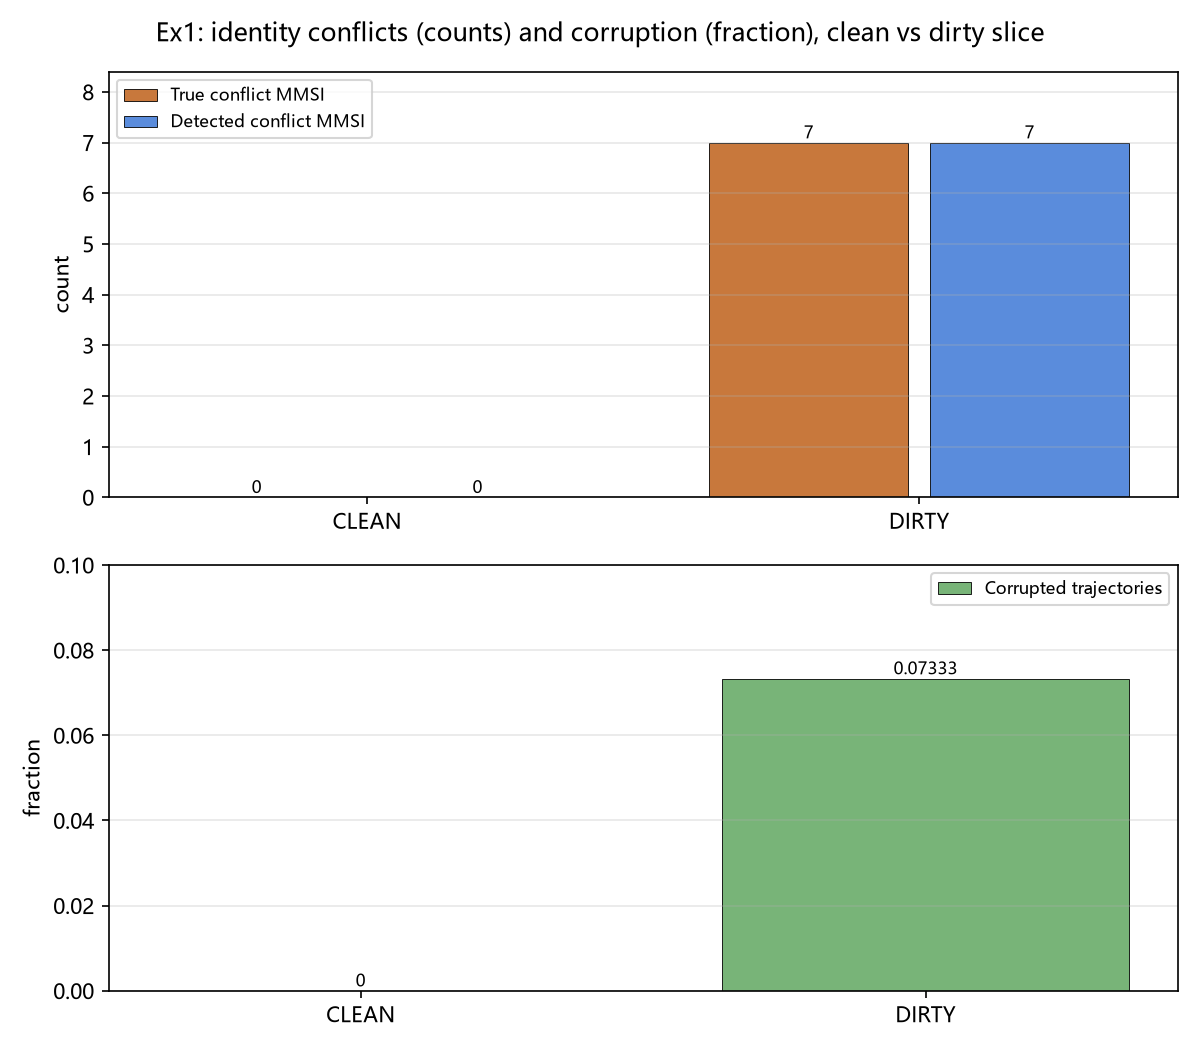
\includegraphics[width=0.76\linewidth]{fig1_identity.png}
\caption{实验一：身份冲突计数与污染轨迹占比（CLEAN vs DIRTY）}\label{f1}
\end{figure}

\subsection{实验二：排序轴假象的因果分解}
\textbf{设置}：单船 360 点 @60 s，真实航速上限 10 kn，假象阈值 $\eta=18$ kn；送达延迟 80\%秒级+15\%分钟级+5\%十分钟级（产生乱序）；2$\times$2 因子：{到达序/事件序}$\times${clean/noisy（$\sigma$=150 m+2 瞬移点）}。

\textbf{结果}（表 2、图 2）：clean+事件序折返与超速严格为 0（断言）；到达序在乱序下必然出现假象；noisy+事件序残余超速 16.7\%。

\textbf{小结}：事件时间排序是消除假象的\emph{必要不充分条件}——排序轴修好后，位置噪声与瞬移点仍独立制造超速，教材把假象单一归因于排序轴不完整。

\begin{table}[htbp]\centering\small
\caption{实验二：2$\times$2 归因（折返/超速段占比）}\label{t2}
\begin{tabular}{lcccc}
\toprule
条件 & 折返·到达序 & 折返·事件序 & 超速·到达序 & 超速·事件序\\
\midrule
clean & 0.1504 & \textbf{0.0000} & 0.1504 & \textbf{0.0000}\\
noisy & 0.2228 & \textbf{0.0000} & 0.3036 & \textbf{0.1671}\\
\bottomrule
\end{tabular}
\end{table}
\begin{figure}[htbp]\centering
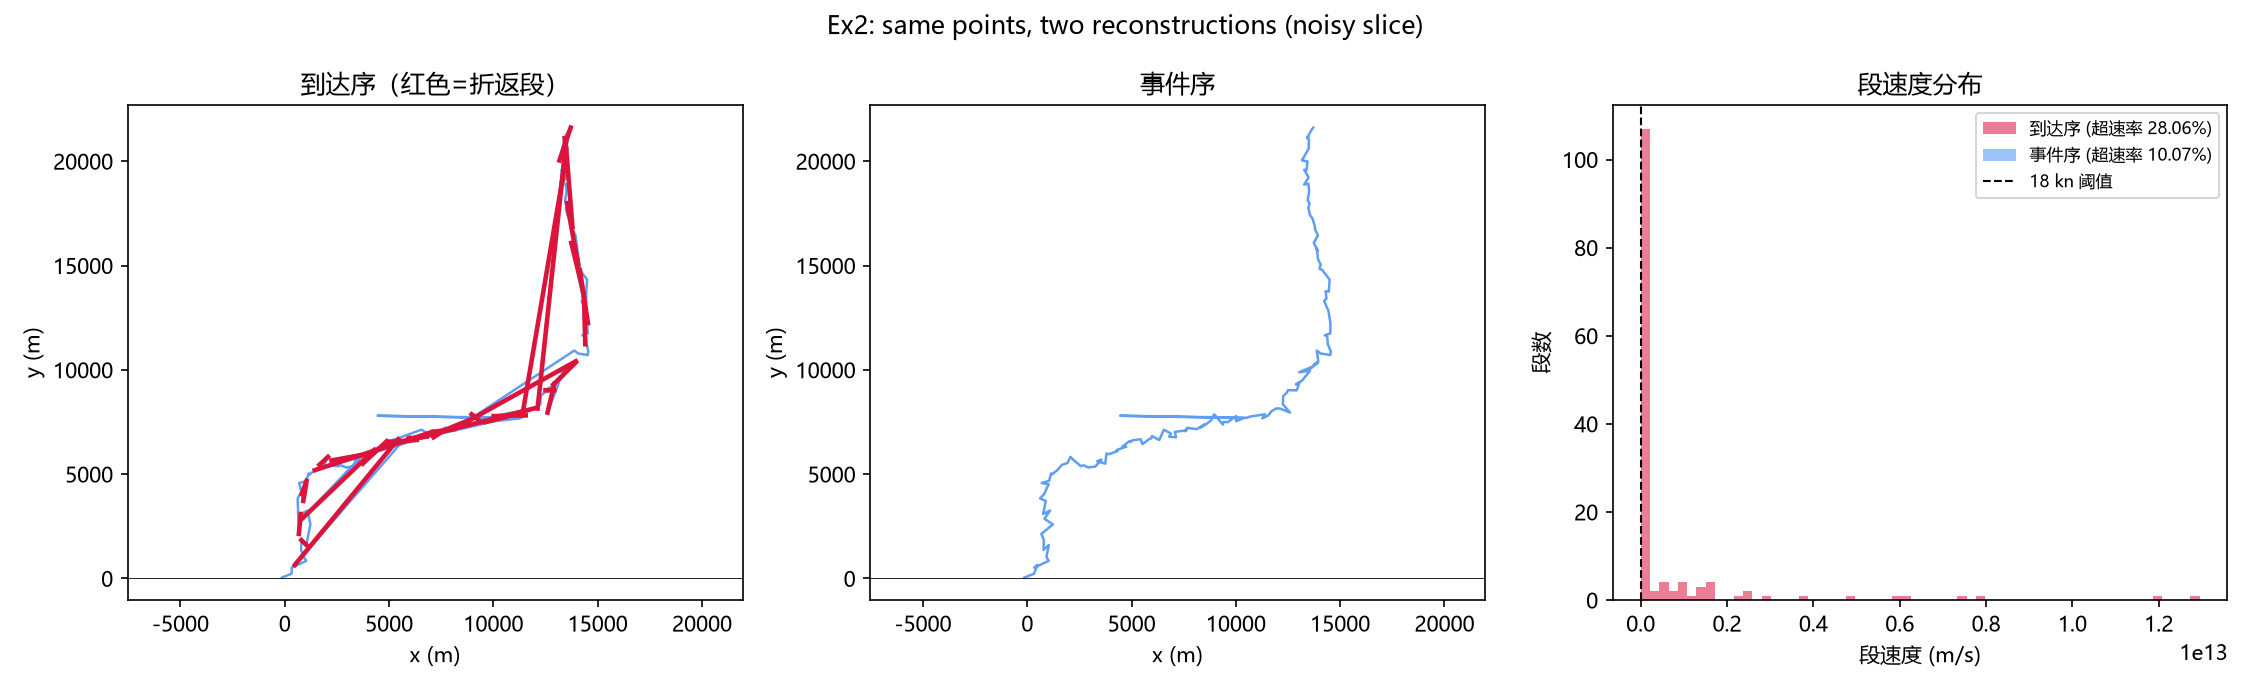
\includegraphics[width=\linewidth]{fig2_sorting.png}
\caption{实验二：同一点集两种重建（到达序红色折返段）与段速度分布}\label{f2}
\end{figure}

\subsection{实验三：双路/重传重复率与幂等键验证}
\textbf{设置}：120 艘 $\times$ 50 条唯一事实（6000 条）；每条副本数 $1+\text{Poisson}(\lambda)$，$\lambda$ 自 0.1 扫描至 1.0（另做 0--1.4 细扫描）；卫星路径占 50\%（延迟 1 min--1 h）。

\textbf{结果}（表 3、图 3）：重复率随拓扑 8.95\%$\to$50.56\%；乱序率稳定约 31\%；幂等键（\mmsi{}, 事件时间, 来源序号）在所有拓扑下恰好恢复 6000/6000（误差 0，断言）。

\textbf{小结}：重复率是接收网拓扑的连续函数而非常数；乱序率由延迟差驱动与副本数无关；键设计自洽性在 15 档拓扑上得到实证。

\begin{table}[htbp]\centering\small
\caption{实验三：重复率与乱序率（$\lambda$=平均附加送达路径数）}\label{t3}
\begin{tabular}{lccccc}
\toprule
$\lambda$ & 唯一事实 & 送达 & 重复率 & 乱序率 & 键恢复\\
\midrule
0.1 & 6000 & 6590 & 8.95\% & 31.55\% & 6000/6000\\
0.5 & 6000 & 9084 & 33.95\% & 31.17\% & 6000/6000\\
1.0 & 6000 & 12\,135 & 50.56\% & 30.94\% & 6000/6000\\
\bottomrule
\end{tabular}
\end{table}
\begin{figure}[htbp]\centering
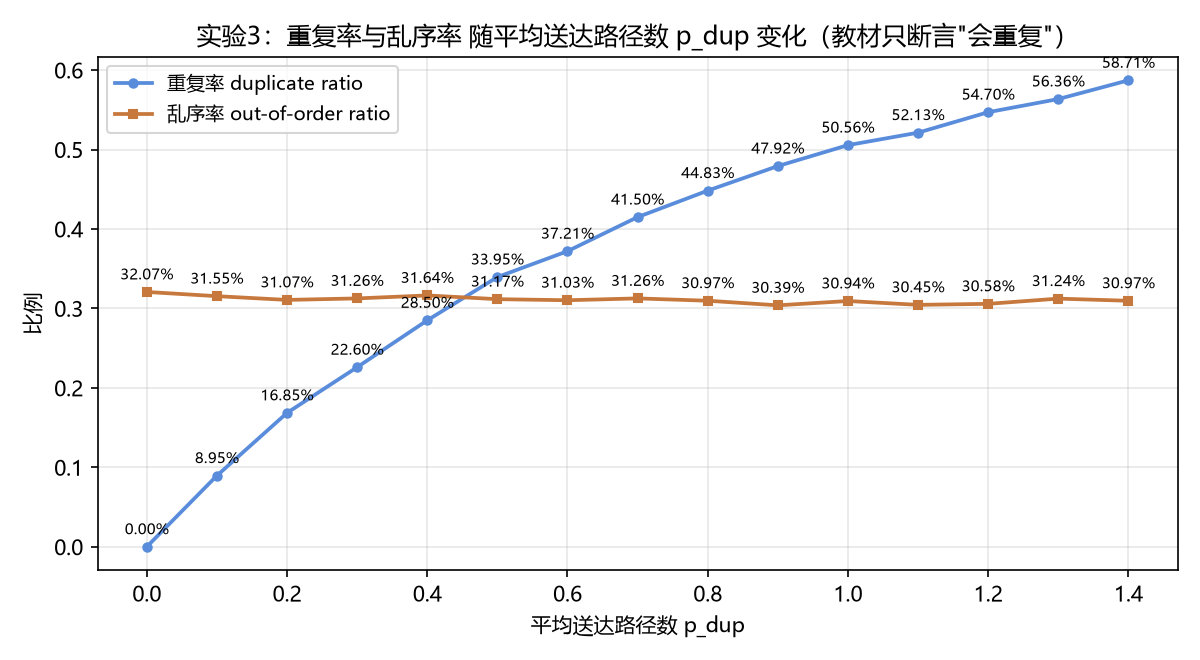
\includegraphics[width=0.8\linewidth]{fig3_duplication.png}
\caption{实验三：重复率与乱序率随平均附加路径数 $\lambda$ 变化}\label{f3}
\end{figure}

\subsection{实验四：真实单船双层验证}
\textbf{设置}：真实单船轨迹（\mmsi{} 210253000，Kattegat，2026-09-26，1657 点）为环境；克隆第二物理船 B（经度 +0.6°$\approx$36 km），注入 3 个``共用''窗（B 改用 A 的 \mmsi{}，396 行）与 1 个``改写''窗（A 改用伪造 \mmsi{}，154 行）；位置/时间/航速全为真实值；登记册以模拟快照实现（公开导出脱敏）。

\textbf{结果}（表 4、图 4）：纯真实基线 0 误报（断言）；位置启发式共用召回 1.00、改写召回 0.00（0/154）；登记册交叉两类召回均 1.00、精度 1.00。

\textbf{小结}：在真实位置与噪声上复现``检测不对称''——同一艘船换个 \mmsi{} 继续播报，纯位置层面彻底失明；独立静态证据把改写召回从 0 补到 1.0。

\begin{table}[htbp]\centering\small
\caption{实验四：真实单船双层验证}\label{t4}
\begin{tabular}{lccc}
\toprule
验证层 & 共用召回 & 改写召回 & 精度\\
\midrule
纯真实单船基线 & --- & --- & 0 flag（断言通过）\\
位置启发式 & 1.00 (396/396) & \textbf{0.00 (0/154)} & 1.00\\
登记册交叉 & 1.00 & 1.00 & 1.00\\
\bottomrule
\end{tabular}
\end{table}
\begin{figure}[htbp]\centering
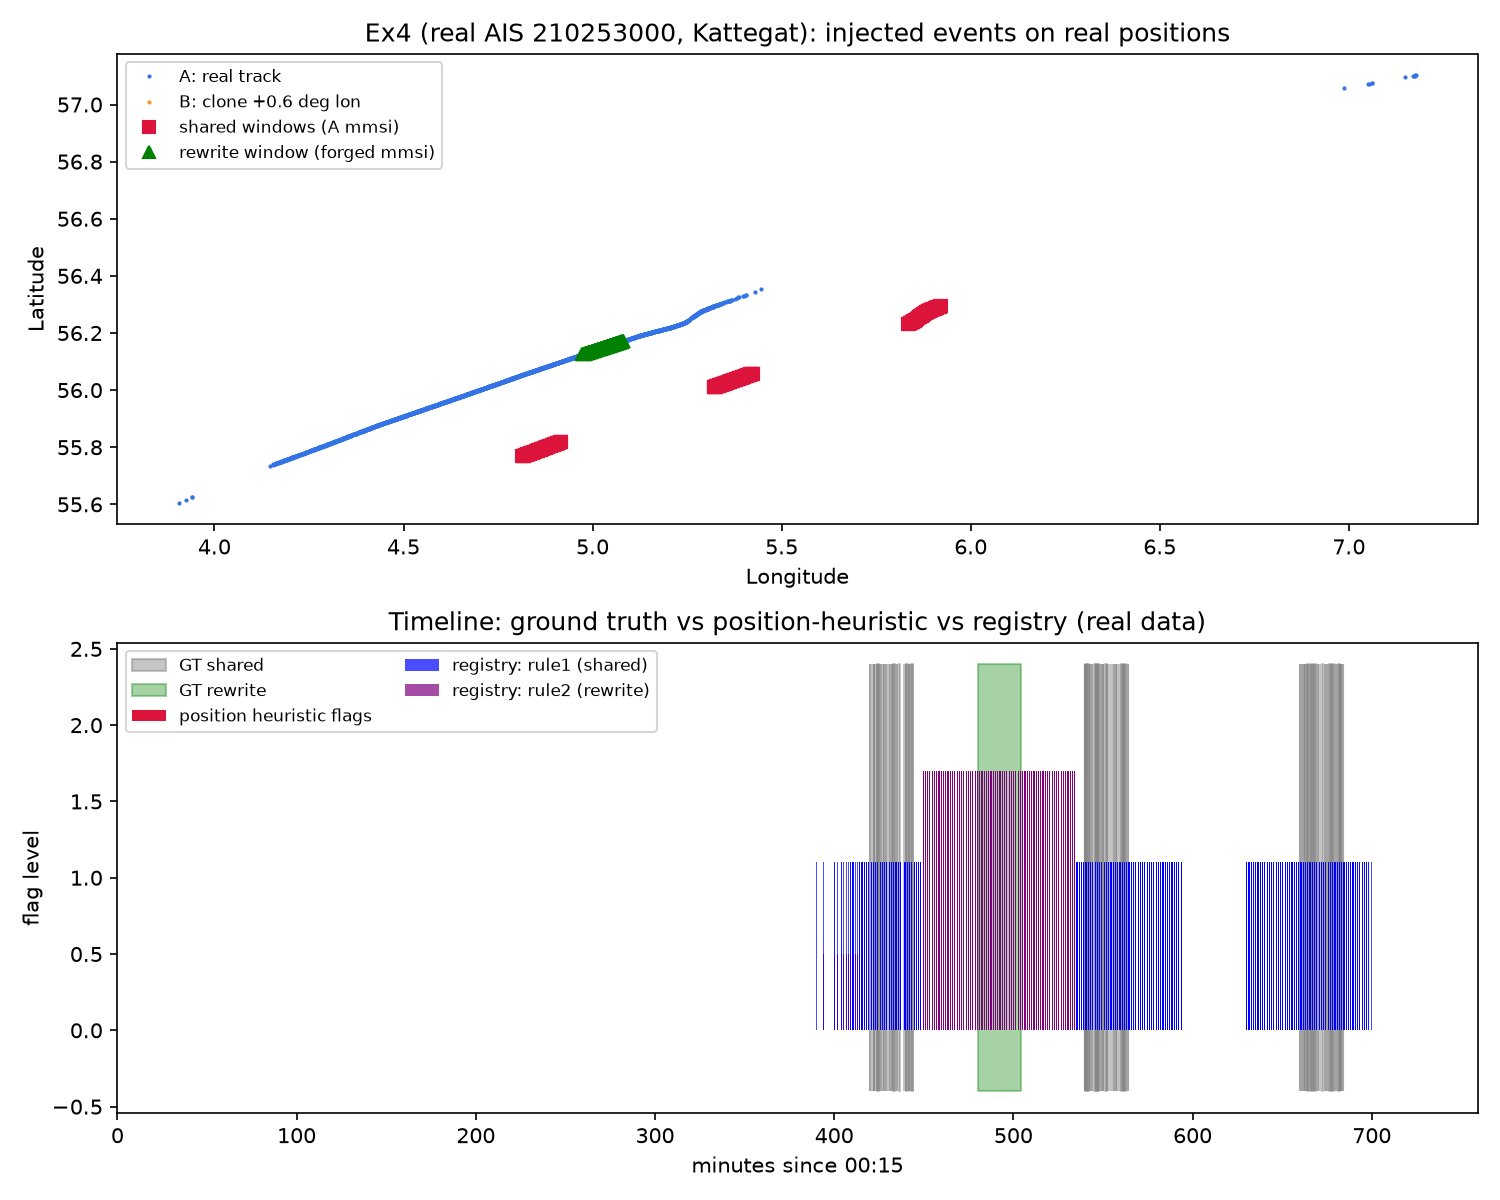
\includegraphics[width=0.9\linewidth]{fig4_realdata.png}
\caption{实验四：真实轨迹上的注入事件（上）与 flag 时间轴对照（下）}\label{f4}
\end{figure}

\subsection{实验五：真实多船快照}
\textbf{设置}：real-noaa（USCG/BOEM/NOAA，CC0），2024-01-01 00:00--00:02:19 全美沿海前 5000 条、4614 船（快照型：386 艘 2 条、其余 1 条），含静态字段。

\textbf{结果}（表 5、图 5）：位置启发式仅 2 个 flag、集中 1 船（\mmsi{} 367373000），而该船恰是第三方审计工具 ais-quality 唯一标记的 position\_jump|speed\_exceeded 对象——两套独立实现收敛；身份一致性（同 \mmsi{} 多 IMO/呼号/船名）为 0；9 例 IMO$\to$多 \mmsi{} 中 6 例占位符伪值、3 例真候选（7222152/8851273/9813644）；IMO 缺失率 57.3\%、呼号 9.0\%。

\textbf{小结}：位置层在``每船 1--2 条''的快照上几乎无判定力，身份层仍工作——再次印证两层时间尺度分工；57.3\% 的 IMO 缺失构成 AIS 盲区的静态事实基线。

\begin{table}[htbp]\centering\small
\caption{实验五：真实多船快照（零注入）}\label{t5}
\begin{tabularx}{\textwidth}{@{}l p{4.6cm} X@{}}
\toprule
指标 & 数值 & 说明\\
\midrule
位置冲突检测 & 2 flag / 1 船（367373000） & 与第三方审计收敛\\
同 \mmsi{} 多 IMO/呼号/船名 & 0 / 0 / 0 & 快照内自洽\\
IMO$\to$多 \mmsi{} & 9（6 占位 + 3 真候选） & 真候选见表 12\\
(MMSI, 时间) 精确重复 & 0 & 入库侧已去重\\
IMO/呼号缺失率 & 57.3\% / 9.0\% & AIS 盲区静态基线\\
\bottomrule
\end{tabularx}
\end{table}
\begin{figure}[htbp]\centering
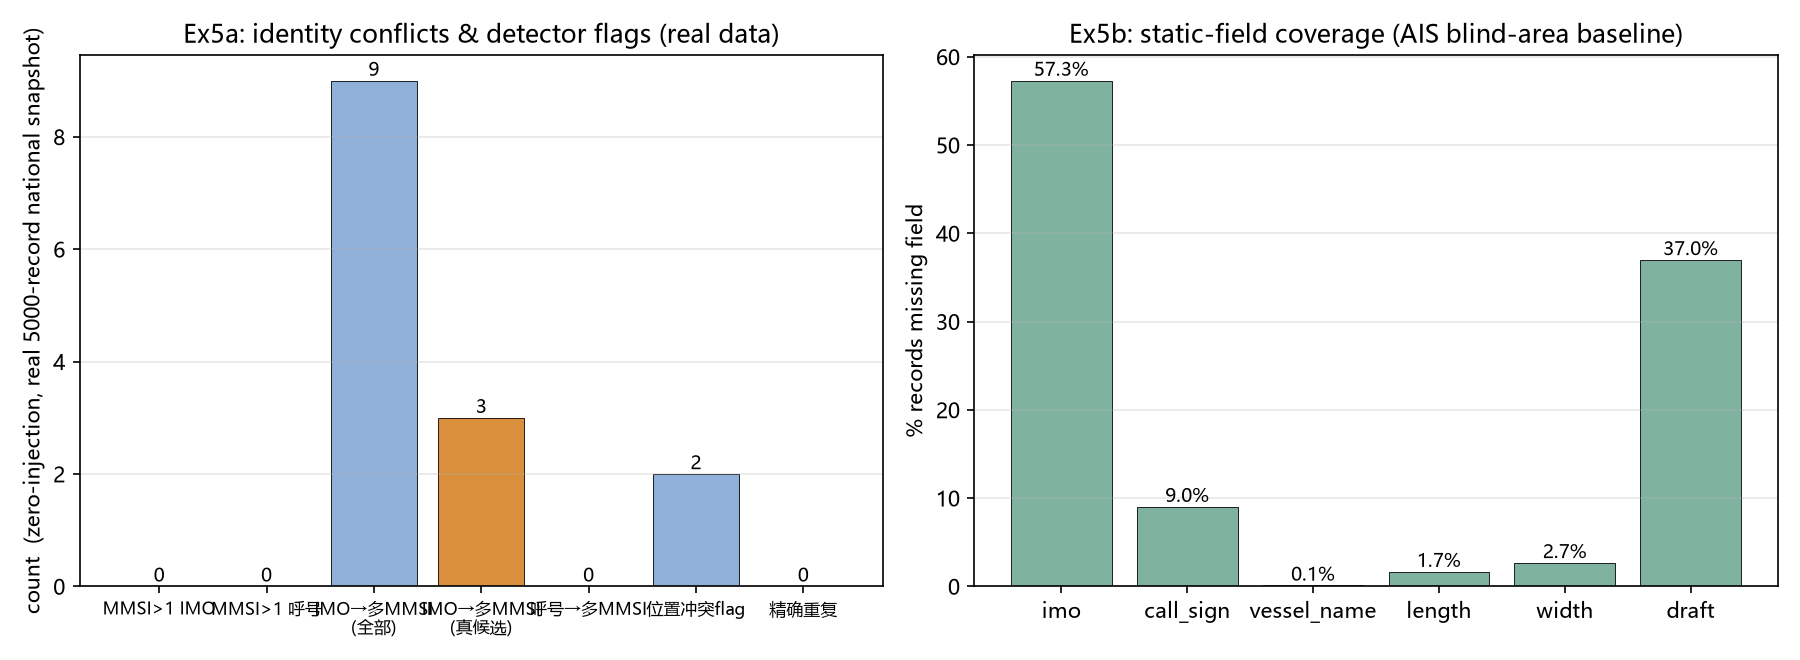
\includegraphics[width=0.9\linewidth]{fig5_realmulti.png}
\caption{实验五：身份冲突信号（左）与静态字段覆盖（右）}\label{f5}
\end{figure}

\subsection{实验六：真实多船轨迹小时窗}
\textbf{设置}：MarineCadastre AIS\_2015\_01\_01，流式扫描 6\,M 行取最繁忙小时窗 2015-01-01 00:00--01:00 UTC：260\,001 行、8072 船、每船中位 28 点。

\textbf{结果}（表 6、图 6）：位置冲突 135 分钟位、集中 5 艘（约 0.06\%），全部为真实瞬移/坏点（如 \mmsi{} 1193046 单段 5708 km/17.9 万节）；其中 \mmsi{} 100000000 不在有效船用编码空间；身份层小时窗内 0 冲突、同呼号$\to$多 \mmsi{} 4 例候选；真实段速中位 0.07 kn、p99.9=32.7 kn、$>$50 kn 占 0.043\%。

\textbf{小结}：轨迹型真实数据上位置层正常工作且抓到的是数据错误与非标准编号；中心发现是两层时间尺度分工：位置层=分钟级瞬移，身份层=跨窗口静态不一致。

\begin{table}[htbp]\centering\small
\caption{实验六：真实多船轨迹小时窗（零注入）}\label{t6}
\begin{tabularx}{\textwidth}{@{}l p{4.6cm} X@{}}
\toprule
指标 & 数值 & 说明\\
\midrule
位置冲突 & 135 分钟位 / 5 船 & 全为瞬移/坏点\\
非标准 \mmsi{} & 100000000 & 不在有效船用编码空间\\
同 \mmsi{} 多 IMO/呼号/船名 & 0 / 0 / 0 & 小时窗内自洽\\
同呼号$\to$多 \mmsi{} & 4 例 & 候选见表 12\\
真实段速 & 中位 0.07；p99.9=32.7；$>$50 kn 占 0.043\% & 瞬移坏点\\
\bottomrule
\end{tabularx}
\end{table}
\begin{figure}[htbp]\centering
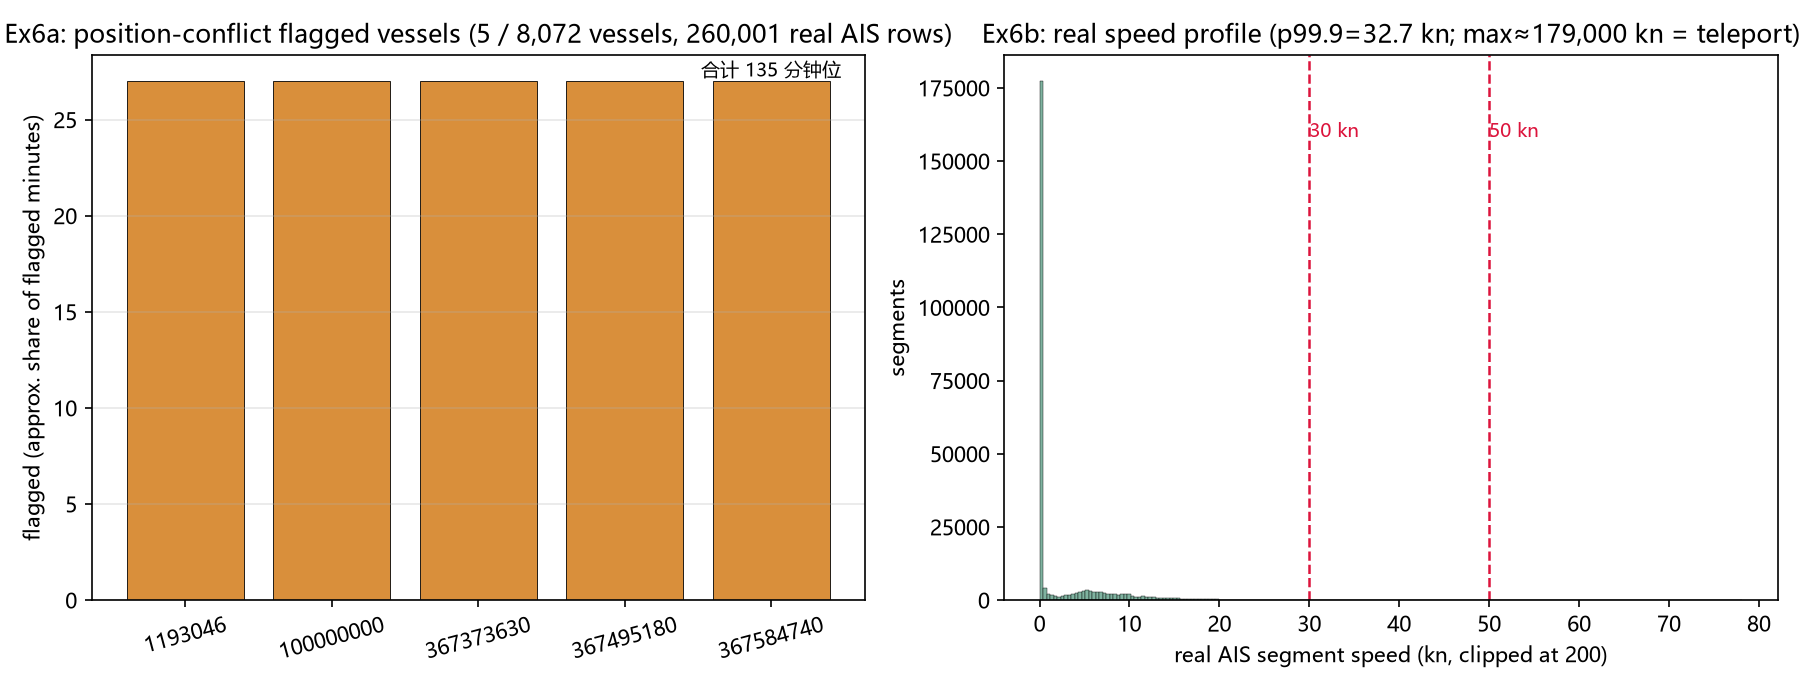
\includegraphics[width=0.9\linewidth]{fig6_mc_traj.png}
\caption{实验六：位置冲突被标船（左）与真实段速剖面（右）}\label{f6}
\end{figure}

\subsection{算法与模型对比}
\textbf{设置}：三个合成切片（TEST-A 更脏 8\%/5\%/2\%；TEST-ADV 近距离同行；TEST-CLEAN 全 0），统一加实时噪声（GPS $\sigma$=600 m + 2\% 瞬移坏点）；六种方法同对同特征对照。

\textbf{结果}（表 7--11）：实体解析对级 F1 0.961（基线）$\to$0.991（CGER）；MMSI 级共享检测，逻辑回归在 TEST-A/ADV 均 (1.00,1.00)、CLEAN 零误警；朴素 GNN 共享召回 0、$\alpha$=0.8 后 PR-AUC 回升至 0.999 但共享召回仍 0；边门控确证机制（GNN PR-AUC 1.0），结构红利落在``门控+连通分量''（共享召回 0$\to$0.833）。

\textbf{小结}：本任务上轻量逐对 + 显式结构是帕累托最优；GNN（朴素或门控）不提供额外价值，其适用前提是``先剔除待判别的跨实体边''。

\begin{table}[htbp]\centering\small
\caption{MMSI 级共享检测精度/召回（真共享数 12/15/0）}\label{t7}
\begin{tabular}{lcccc}
\toprule
方法 & TEST-A & TEST-ADV & TEST-CLEAN & 说明\\
\midrule
启发式 30 km/30 min & (1.00,1.00) & (1.00,1.00) & (0,0) & 二元 flag\\
CGER（手调阈值） & (0.435,0.833) & (0.381,0.533) & (0,0) & 物理模型\\
逻辑回归（仅运动） & (1.00,1.00) & (1.00,1.00) & (0,0) & ECE$\approx$0\\
朴素 GNN & (0,0) & (0,0) & (0,0) & 共享召回 0\\
GNN（$\alpha$=0.8） & (0,0) & (0,0) & (0,0) & AUC 0.999\\
门控+UF & (0.435,0.833) & (0.381,0.533) & (0,0) & 结构红利\\
\bottomrule
\end{tabular}
\end{table}
\begin{table}[htbp]\centering\small
\caption{实体解析对级指标（合成 DIRTY 真值）}\label{t8}
\begin{tabular}{lccc}
\toprule
方法 & 精度 & 召回 & F1\\
\midrule
MMSI 即实体（基线） & 0.957 & 0.966 & 0.961\\
CGER 仅同 \mmsi{} & 0.986 & 0.962 & 0.974\\
CGER 完整（双条件桥接） & 0.987 & 0.996 & \textbf{0.991}\\
\bottomrule
\end{tabular}
\end{table}
\begin{table}[htbp]\centering\small
\caption{学习模型（逻辑回归，仅运动特征）}\label{t9}
\begin{tabular}{lccccc}
\toprule
切片 & PR-AUC & 对级 F1 & ECE & 共享 P & 共享 R\\
\midrule
TEST-A & 1.000 & 1.000 & 0.001 & 1.00 & 1.00\\
TEST-ADV & 0.998 & 0.996 & 0.006 & 1.00 & 1.00\\
TEST-CLEAN & 1.000 & 1.000 & 0.001 & 0 & 0\\
\bottomrule
\end{tabular}
\end{table}
\begin{table}[htbp]\centering\small
\caption{GNN 负结果与 $\alpha$ 消融（PR-AUC/F1/ECE/共享 P/R，TEST-A）}\label{t10}
\begin{tabular}{lcccc}
\toprule
方法 & PR-AUC & 对级 F1 & ECE & 共享 P/R\\
\midrule
朴素 GNN（均值聚合） & 0.931 & 0.963 & 0.065 & (0,0)\\
GNN（$\alpha$=0.8） & 0.999 & 0.963 & 0.065 & (0,0)\\
\bottomrule
\end{tabular}
\end{table}
\begin{table}[htbp]\centering\small
\caption{边门控验证（TEST-A）}\label{t11}
\begin{tabular}{lcccc}
\toprule
方法 & PR-AUC & 对级 F1 & 共享 P/R & 说明\\
\midrule
朴素 GNN & 0.999 & 0.963 & (0,0) & 对照\\
GNN（门控后） & 1.000 & 0.963 & (0,0) & 排序恢复\\
门控+连通分量 & --- & 0.993 & (0.435,0.833) & 结构红利落点\\
\bottomrule
\end{tabular}
\end{table}

\subsection{登记册裁决：统计信号升级为判决证据}
\textbf{设置}：以两片独立真实切片（NOAA 2024 与 MarineCadastre 2015）按 IMO/呼号建登记簿，逐条交叉裁决实验五/六的拆分候选；同时统计跨年 \mmsi{} 复用换名。

\textbf{结果}（表 12）：7/7 候选全部 CONFLICT（同一标识下出现不同船名）；跨年复用 \mmsi{} 1401 个中 155 个换名（11.06\%）。

\textbf{小结}：从``统计信号''到``带船名/年份的证据链''是质的升级；并发冲突更可能是配置/拷贝错误，跨年换名多为 \mmsi{} 正常回收，均已在口径声明中标明。

\begin{table}[htbp]\centering\scriptsize
\caption{登记册交叉裁决（7/7 CONFLICT）}\label{t12}
\begin{tabular}{@{}p{1.7cm}p{10.8cm}c@{}}
\toprule
标识 & 冲突的船名（年/\mmsi{}） & 裁决\\
\midrule
IMO7222152 & OLIVIA ROSE(24/367644590)、MARNE B(24/367501920)、KIMBERLY JANE(15) & CONFLICT\\
IMO8851273 & SABINE PILOT(24/366896250)、LAKE CHARLES(24/367456860) & CONFLICT\\
IMO9813644 & ROSEMARY MCALLISTER(24/368006020)、RTA1(24/368041830) & CONFLICT\\
WCW6340 & BEAVER(15/338048556)、DUTRA DB 24(15/338048555) & CONFLICT\\
WDF8768 & FLOAT PLANT INGRAM(15/367498360)、CHARLES B. HOLMAN(15/366963290) & CONFLICT\\
WSL5671 & RACHAEL(24+15/338124433)、CAPTAIN MARLON(15/338132812) & CONFLICT\\
WZX4855 & GLADYS FORD(15/528155000)、MS NANCY C(15/614211000) & CONFLICT\\
\bottomrule
\end{tabular}
\end{table}

\subsection{初步结论}
（1）教材三条定性结论已改写为带条件的定量命题并通过真值对账；（2）``轻量逐对 + 显式结构''在本任务是帕累托最优，GNN 负优化及其机制解释给出可引用的适用前提；（3）\mmsi{} 身份冲突在两片独立真实切片上真实存在（7/7 候选冲突、跨年换名率 11.06\%）。

\section{课题进度安排}
\subsection{时间计划}
\begin{table}[htbp]\centering\small
\caption{课题进度安排（两周）}\label{tsched}
\begin{tabular}{@{}p{2.2cm}p{9.2cm}c@{}}
\toprule
阶段 & 主要任务 & 完成标志\\
\midrule
第 1--3 天 & 三条结论命题化、合成实验 1--3、断言体系 & 表 1--3 与图 1--3\\
第 4--6 天 & CGER 算法、参数敏感性、学习模型 & 表 8--9\\
第 7--9 天 & GNN 负结果、$\alpha$ 消融、边门控闭环 & 表 10--11\\
第 10--12 天 & 真实单船/快照/轨迹三切片验证 & 表 4--6、图 4--6\\
第 13--14 天 & 登记册裁决、仓库整理、报告成文与自查 & 表 12、可复现清单\\
\bottomrule
\end{tabular}
\end{table}

\subsection{里程碑与检查点}
里程碑一（第 3 天）：合成三命题全部通过断言；里程碑二（第 6 天）：算法与学习模型在 TEST-A 达到既定指标；里程碑三（第 9 天）：负结果闭环（$\alpha$ 消融 + 边门控）；里程碑四（第 12 天）：真实三切片交叉验证完成；里程碑五（第 14 天）：登记册裁决 + 仓库与报告交付。

\section{课题预期成果}
\subsection{课题研究特色}
本课题的特色是``一个创新点、九要素闭环、全链路可复现''：（1）不主张新 SOTA 算法，而把定性结论变成带条件的定量命题；（2）真值注入同时承担验证与训练双重职能，避免自证循环；（3）诚实报告负结果，并以 $\alpha$ 消融与边门控给出机制解释与适用边界；（4）所有数字可一键复现、关键断言内建。

\subsection{预期研究成果}
（1）一份完整实验报告（本文）；(2) 一套可复现代码与数据切片（含 9 个脚本、6 张图、12 张表）；(3) 一个公开 GitHub 仓库（README、复现命令、口径合同、许可说明）；(4) 一份``单一创新点九要素核查表''用于提交自查。

\section{参考文献}
\begin{thebibliography}{9}\small
\bibitem{textbook} 课程教材. 海洋大数据：工程与治理，\S3.5.2 时空主键与乱序修复[Z]. 出版信息待补.
\bibitem{gfw2024} Kroodsma D A, et al. Satellite mapping reveals extensive industrial activity at sea[J]. Nature, 2024, 625: 600-608.
\bibitem{imo2023} IMO. Resolution A.1192(33): Measures to prevent the engagement of substandard and non-compliant shipping[R]. 2023.
\bibitem{kallista} Lloyd's List. Tanked: identity theft of a VLCC hits sanctions enforcement[N]. 2025-12.
\bibitem{noaa} USCG/BOEM/NOAA. Nationwide Automatic Identification System (AIS)[DS]. MarineCadastre.
\bibitem{aisquality} ais-quality: open-source AIS data quality auditing[CP/OL]. GitHub.
\bibitem{repo} 本文配套 GitHub 仓库：\url{\ghrepo}[CP/OL].
\end{thebibliography}

\newpage
\section*{附录：可复现性与提交核查清单}
\addcontentsline{toc}{section}{附录：可复现性与提交核查清单}
\noindent\small\textbf{GitHub 仓库：}\url{\ghrepo}\normalsize\quad（封面与本节两处显著位置）

复现命令（逐条执行即可）：
\begin{verbatim}
python run_all.py              # 实验1-3（合成）
python ex4_realdata.py         # 实验4 真实单船
python ex5_realmulti.py        # 实验5 多船快照
python ex6_mc_traj.py          # 实验6 多船轨迹
python algo_cger.py            # CGER 算法
python model_link.py           # 学习链接预测
python model_gnn.py            # GNN 负结果
python model_ggnn.py           # 边门控 GNN
python adjudicate_registry.py  # 登记册裁决
\end{verbatim}
产物位于 \texttt{results/}：CSV/JSON（原始数字）、fig1--6（本文插图）、results\_summary.md。代码内建断言自动验证（clean 零假象、幂等键精确恢复、真实单船零误报），复跑即自检。

\noindent\textbf{参数与口径合同}：见仓库 README 与 results\_summary.md；关键参数为种子 42、$V_{\max}$=45 kn、$R_0$=1 km、$C_{\max}$=25 km、$\Delta t\le$1 h、GPS $\sigma$=600 m + 2\% 瞬移、$\alpha$=0.8、$\tau$=0.2。

\noindent\textbf{数据溯源与许可}：real-noaa（USCG/BOEM/NOAA，CC0）；MarineCadastre（美国沿海公开数据）；单船轨迹（GitHub 公开演示数据，身份脱敏）；EnvShip-Bench 因需登录未采用。

\noindent\textbf{AI 使用声明}：数据获取、仿真、绘图与全部数值均由仓库内 Python 脚本生成；关键数值均内建断言自动复核；大语言模型仅用于脚本编写与文本润色，不参与结论判定。

\end{document}
